\documentclass[aspectratio=169,12pt]{beamer}
\usetheme{Madrid}
\usecolortheme{dolphin}
\usefonttheme{professionalfonts}
\setbeamertemplate{navigation symbols}{}
\setbeamertemplate{footline}{}

\usepackage[T1]{fontenc}
\usepackage[utf8]{inputenc}
\usepackage{graphicx}
\usepackage{amsmath,amssymb}
\usepackage{hyperref}
\usepackage{siunitx}
\usepackage{physics}
\usepackage{braket}
\usepackage{tikz}

\title[Chapter 4]{Chapter 7: Platforms implementing quantum computers}
\author{JAMOTTE Maxime, SCHOONEN Cédric}
\institute{Digital Learning Hub}
\date{}

\begin{document}

\begin{frame}
  \titlepage
\end{frame}

\begin{frame}
    \begin{itemize}
        \item Classical platform\\~\\
        \item Quantum platforms
    \end{itemize}
\end{frame}

\begin{frame}{Classical platform: silicon CMOS}
\begin{itemize}
    \item Classical computers use \textbf{CMOS} circuits fabricated on \textbf{silicon}.
    \item A bit is encoded by a \textbf{voltage level}:
    \[
        0 = \text{low voltage}, \qquad 1 = \text{high voltage}.
    \]
    \item The fundamental component is the \textbf{transistor}:
    \begin{itemize}
        \item open channel = 1,
        \item closed channel = 0.
    \end{itemize}
    \item Logic gates are built by connecting multiple transistors:
    \begin{itemize}
        \item NOT = 1 PMOS + 1 NMOS,
        \item AND/OR = transistors in series or parallel,
        \item NAND/NOR = fundamental building blocks of processors.
    \end{itemize}
    \item Everything is fabricated by \textbf{photolithography} on doped silicon.
\end{itemize}
\end{frame}



\begin{frame}{Quantum platforms}
\begin{itemize}
    \item Superconducting qubits\\~\\
    \item Neutral atoms\\~\\
    \item Trapped ions\\~\\
\end{itemize}
\end{frame}

\begin{frame}{Superconducting qubits (IBM, Google,...)}
\begin{columns}[T]
\begin{column}{0.6\textwidth}
\begin{itemize}
    \item \textbf{Superconducting circuits} (LC + Josephson junction) behave 
    like \textbf{artificial atoms}.\\~\\
    \item The first two energy levels form the qubit:
    \[
        |0\rangle = \text{ground state},
        |1\rangle = \text{first excited state}.
    \]
    \item Quantum operations are performed with \textbf{microwave laser pulses}.
    ~\\~\\
    \item Different frequencies to access other energy levels.
\end{itemize}
\end{column}
\begin{column}{0.4\textwidth}
\centering
\begin{tikzpicture}
    \node[inner sep=0] (img) {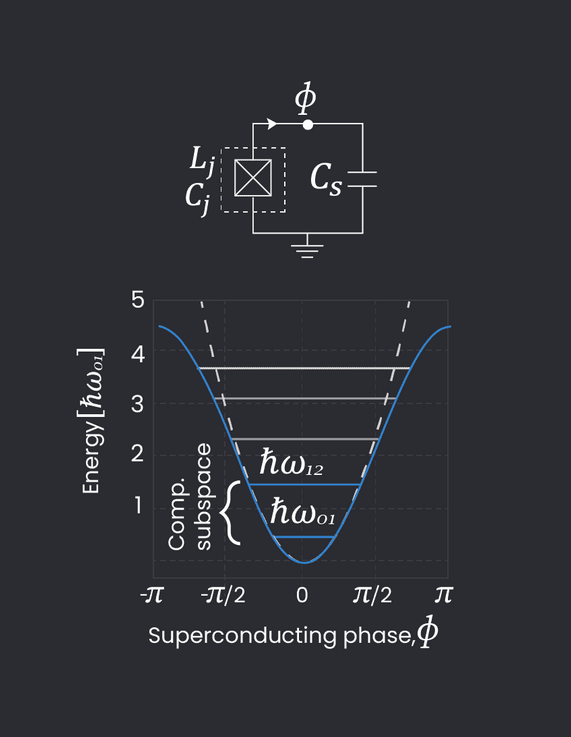
\includegraphics[width=0.8\linewidth]{../figures/qubit_SC.png}};
    \node[anchor=south east,text=white,font=\scriptsize] at (img.south east) {Pierre Guichard};
\end{tikzpicture}
\end{column}
\end{columns}
\end{frame}

\begin{frame}{Trapped ions (Quantinuum, IonQ, Innsbruck / AQT)}
\begin{columns}[T]
\begin{column}{0.6\textwidth}
\begin{itemize}
    \item Individual \textbf{ions} (e.g.: Yb\(^+\), Ca\(^+\)) are aligned in an \textbf{electromagnetic trap}.
    \item The qubit is encoded in two stable \textbf{internal levels} of the atom:
    \[
        |0\rangle = \text{hyperfine level A},\ |1\rangle = \text{hyperfine level B}.
    \]
    \item Quantum operations via \textbf{laser pulses}:
    \begin{itemize}
        \item single-qubit rotations,
        \item two-qubit gates via \textbf{collective vibrational mode}.
    \end{itemize}
\end{itemize}
\end{column}
\begin{column}{0.4\textwidth}
\centering
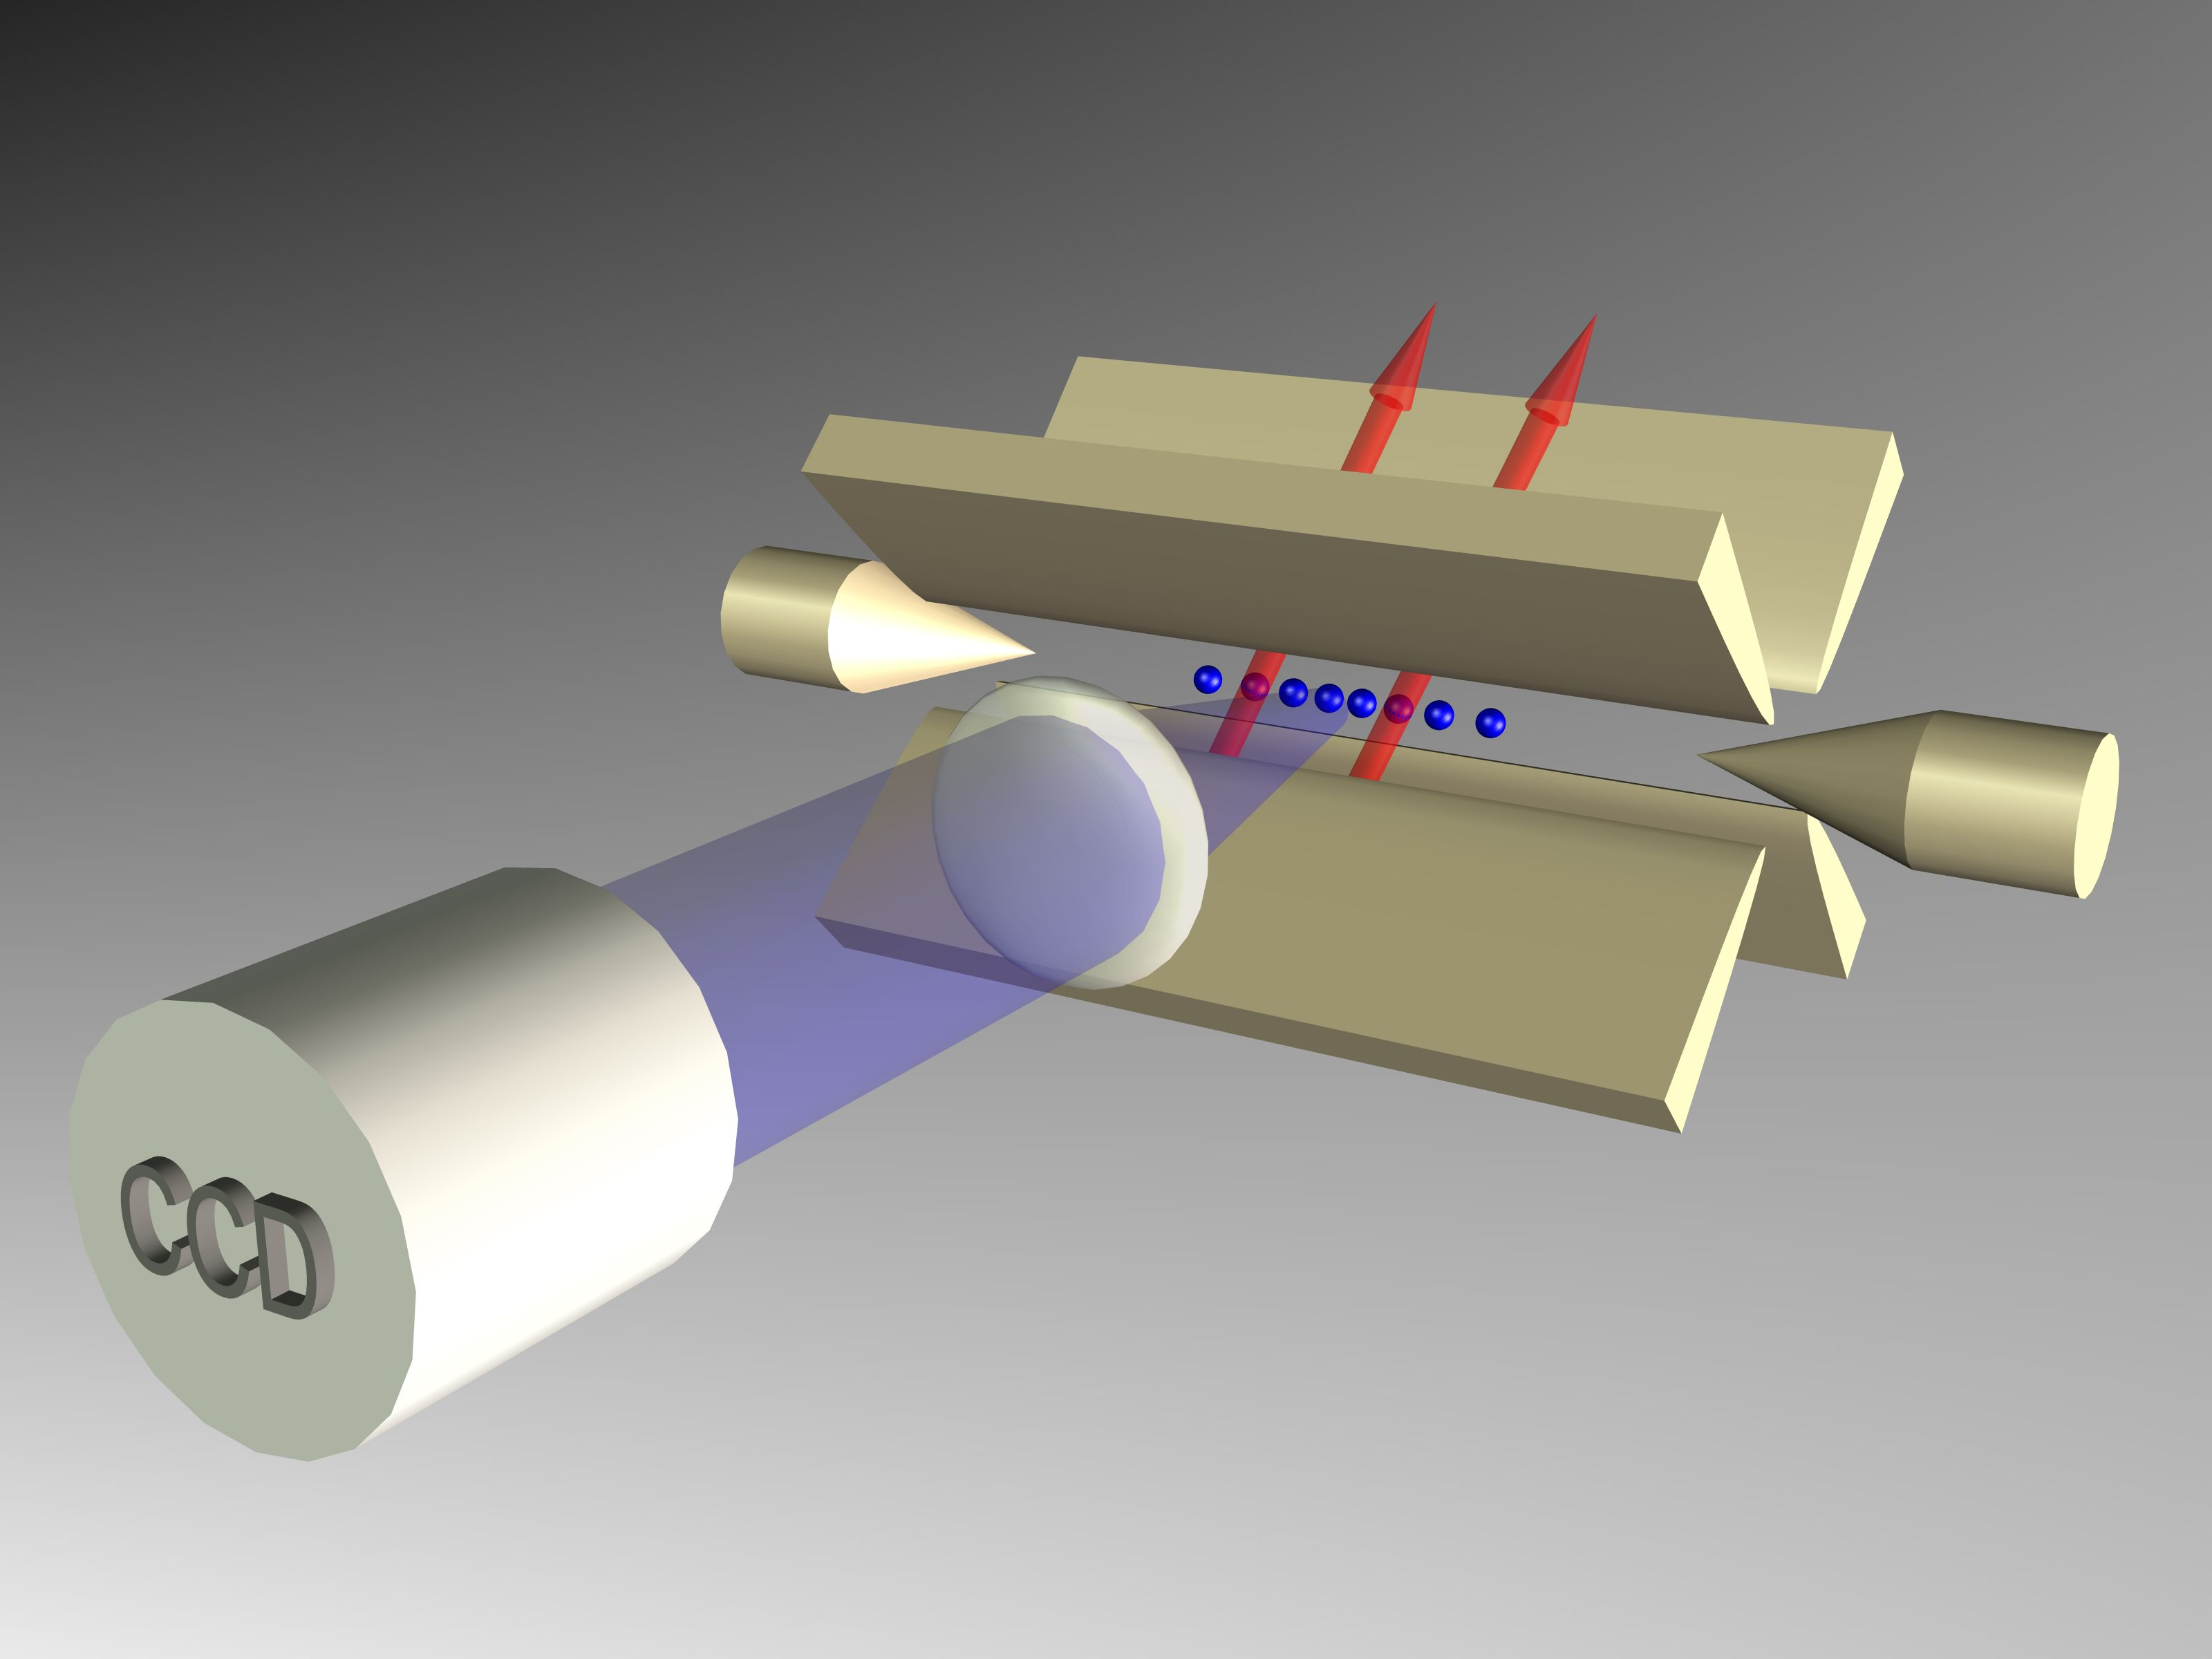
\includegraphics[width=0.8\linewidth]{../figures/ion_trap.jpg}
\end{column}
\end{columns}
\end{frame}

\begin{frame}{Neutral atoms (Pasqal, QuEra, ColdQuanta)}
\begin{columns}[T]
\begin{column}{0.6\textwidth}
\begin{itemize}
    \item Neutral atoms (Rb, Cs) are trapped one by one in \textbf{optical tweezers}.\\~\\
    \item The qubit corresponds to two \textbf{hyperfine levels} of the atom:
    \[
        |0\rangle = \text{hyperfine A}, \qquad |1\rangle = \text{hyperfine B}.
    \]
    \item Quantum operations via \textbf{laser pulses}:
    \begin{itemize}
        \item single-qubit operations,
        \item controlled interactions via \textbf{Rydberg blockade} (highly excited state).\\~\\
    \end{itemize}
    \item The atoms can be \textbf{freely moved} to reconfigure the processor geometry.
\end{itemize}
\end{column}
\begin{column}{0.4\textwidth}
\centering
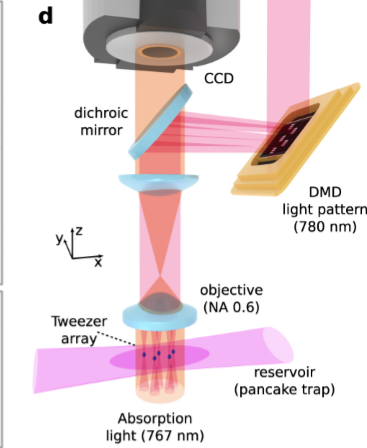
\includegraphics[width=0.8\linewidth]{../figures/atomes_neutres.png}
\end{column}
\end{columns}
\end{frame}

\begin{frame}{End of chapter 7}
    \centering
 Other platforms exist: Spins in semiconductors and photonics.
\end{frame}


\end{document}
